
%% bare_jrnl.tex
%% V1.4a
%% 2014/09/17
%% by Michael Shell
%% see http://www.michaelshell.org/
%% for current contact information.
%%
%% This is a skeleton file demonstrating the use of IEEEtran.cls
%% (requires IEEEtran.cls version 1.8a or later) with an IEEE
%% journal paper.
%%
%% Support sites:
%% http://www.michaelshell.org/tex/ieeetran/
%% http://www.ctan.org/tex-archive/macros/latex/contrib/IEEEtran/
%% and
%% http://www.ieee.org/

%%*************************************************************************
%% Legal Notice:
%% This code is offered as-is without any warranty either expressed or
%% implied; without even the implied warranty of MERCHANTABILITY or
%% FITNESS FOR A PARTICULAR PURPOSE! 
%% User assumes all risk.
%% In no event shall IEEE or any contributor to this code be liable for
%% any damages or losses, including, but not limited to, incidental,
%% consequential, or any other damages, resulting from the use or misuse
%% of any information contained here.
%%
%% All comments are the opinions of their respective authors and are not
%% necessarily endorsed by the IEEE.
%%
%% This work is distributed under the LaTeX Project Public License (LPPL)
%% ( http://www.latex-project.org/ ) version 1.3, and may be freely used,
%% distributed and modified. A copy of the LPPL, version 1.3, is included
%% in the base LaTeX documentation of all distributions of LaTeX released
%% 2003/12/01 or later.
%% Retain all contribution notices and credits.
%% ** Modified files should be clearly indicated as such, including  **
%% ** renaming them and changing author support contact information. **
%%
%% File list of work: IEEEtran.cls, IEEEtran_HOWTO.pdf, bare_adv.tex,
%%                    bare_conf.tex, bare_jrnl.tex, bare_conf_compsoc.tex,
%%                    bare_jrnl_compsoc.tex, bare_jrnl_transmag.tex
%%*************************************************************************


% *** Authors should verify (and, if needed, correct) their LaTeX system  ***
% *** with the testflow diagnostic prior to trusting their LaTeX platform ***
% *** with production work. IEEE's font choices and paper sizes can       ***
% *** trigger bugs that do not appear when using other class files.       ***                          ***
% The testflow support page is at:
% http://www.michaelshell.org/tex/testflow/



\documentclass[journal]{IEEEtran}
%
% If IEEEtran.cls has not been installed into the LaTeX system files,
% manually specify the path to it like:
% \documentclass[journal]{../sty/IEEEtran}





% Some very useful LaTeX packages include:
% (uncomment the ones you want to load)


% *** MISC UTILITY PACKAGES ***
%
%\usepackage{ifpdf}
% Heiko Oberdiek's ifpdf.sty is very useful if you need conditional
% compilation based on whether the output is pdf or dvi.
% usage:
% \ifpdf
%   % pdf code
% \else
%   % dvi code
% \fi
% The latest version of ifpdf.sty can be obtained from:
% http://www.ctan.org/tex-archive/macros/latex/contrib/oberdiek/
% Also, note that IEEEtran.cls V1.7 and later provides a builtin
% \ifCLASSINFOpdf conditional that works the same way.
% When switching from latex to pdflatex and vice-versa, the compiler may
% have to be run twice to clear warning/error messages.






% *** CITATION PACKAGES ***
%
\usepackage{cite}
% cite.sty was written by Donald Arseneau
% V1.6 and later of IEEEtran pre-defines the format of the cite.sty package
% \cite{} output to follow that of IEEE. Loading the cite package will
% result in citation numbers being automatically sorted and properly
% "compressed/ranged". e.g., [1], [9], [2], [7], [5], [6] without using
% cite.sty will become [1], [2], [5]--[7], [9] using cite.sty. cite.sty's
% \cite will automatically add leading space, if needed. Use cite.sty's
% noadjust option (cite.sty V3.8 and later) if you want to turn this off
% such as if a citation ever needs to be enclosed in parenthesis.
% cite.sty is already installed on most LaTeX systems. Be sure and use
% version 5.0 (2009-03-20) and later if using hyperref.sty.
% The latest version can be obtained at:
% http://www.ctan.org/tex-archive/macros/latex/contrib/cite/
% The documentation is contained in the cite.sty file itself.






% *** GRAPHICS RELATED PACKAGES ***
%
\ifCLASSINFOpdf
   \usepackage[pdftex]{graphicx}
  % declare the path(s) where your graphic files are
   \graphicspath{{./figs/}{./figs/}}
  % and their extensions so you won't have to specify these with
  % every instance of \includegraphics
   \DeclareGraphicsExtensions{.pdf,.jpeg,.png}
\else
  % or other class option (dvipsone, dvipdf, if not using dvips). graphicx
  % will default to the driver specified in the system graphics.cfg if no
  % driver is specified.
  % \usepackage[dvips]{graphicx}
  % declare the path(s) where your graphic files are
  % \graphicspath{{../eps/}}
  % and their extensions so you won't have to specify these with
  % every instance of \includegraphics
  % \DeclareGraphicsExtensions{.eps}
\fi
% graphicx was written by David Carlisle and Sebastian Rahtz. It is
% required if you want graphics, photos, etc. graphicx.sty is already
% installed on most LaTeX systems. The latest version and documentation
% can be obtained at: 
% http://www.ctan.org/tex-archive/macros/latex/required/graphics/
% Another good source of documentation is "Using Imported Graphics in
% LaTeX2e" by Keith Reckdahl which can be found at:
% http://www.ctan.org/tex-archive/info/epslatex/
%
% latex, and pdflatex in dvi mode, support graphics in encapsulated
% postscript (.eps) format. pdflatex in pdf mode supports graphics
% in .pdf, .jpeg, .png and .mps (metapost) formats. Users should ensure
% that all non-photo figures use a vector format (.eps, .pdf, .mps) and
% not a bitmapped formats (.jpeg, .png). IEEE frowns on bitmapped formats
% which can result in "jaggedy"/blurry rendering of lines and letters as
% well as large increases in file sizes.
%
% You can find documentation about the pdfTeX application at:
% http://www.tug.org/applications/pdftex

%SKA added packages
\usepackage{xcolor}
\usepackage{tcolorbox}
\tcbuselibrary{breakable}
\usepackage{soul}
\usepackage{color}
\usepackage[normalem]{ulem}
%\usepackage{tikz}
%\usetikzlibrary{external}
%\tikzexternalize[prefix=figs/]
%\usepackage{lmodern}
%\usepackage{pgfplots}
%\pgfplotsset{compat=1.12}
%\pgfplotsset{my style/.append style={axis x line=middle, axis y line=middle, xlabel={$x$}, ylabel={$y$}, axis equal }}
%\pgfplotscreateplotcyclelist{my color}{%
%solid, every mark/.append style={solid, fill=myblue}, mark=*\\%
%solid, every mark/.append style={solid, fill=mygreen}, mark=square*\\%
%solid, every mark/.append style={solid, fill=myred}, mark=diamond*\\%
%solid, every mark/.append style={solid, fill=peru}, mark=triangle*\\%
%}
\definecolor{bblue}{HTML}{4F81BD}
\definecolor{rred}{HTML}{C0504D}
\definecolor{ggreen}{HTML}{9BBB59}
\definecolor{ppurple}{HTML}{9F4C7C}
\definecolor{royalblue}{HTML}{4169E1}
\definecolor{myred}{HTML}{F75B5B}
\definecolor{mygreen}{HTML}{00AD6B}
\definecolor{myblue}{HTML}{1E90FF}
\definecolor{peru}{HTML}{CD853F}
\usepackage{setspace}
\pdfminorversion=4
\newcommand{\factor}{\ensuremath{\textrm{x}\,}}
\newcommand{\myhl}{\bgroup\markoverwith{\textcolor{blue!20}{\rule[-.5ex]{2pt}{2.5ex}}}\ULon}
\newsavebox\IBoxA \newsavebox\IBoxB \newsavebox\IBoxC \newlength\IHeight
\newcommand\TwoFig[6]{% Image1 Caption1 Label1 Image2 ...
  \sbox\IBoxA{\includegraphics[width=0.45\textwidth]{#1}}
  \sbox\IBoxB{\includegraphics[width=0.45\textwidth]{#4}}%
  \ifdim\ht\IBoxA>\ht\IBoxB
    \setlength\IHeight{\ht\IBoxB}\else\setlength\IHeight{\ht\IBoxA}\fi%
  \begin{figure*}[!htb]
  \minipage[t]{0.45\textwidth}\centering
  \includegraphics[height=\IHeight]{#1}
  \caption{#2}\label{#3}
  \endminipage\hfill
  \addtocounter{figure}{-1}
  \minipage[t]{0.45\textwidth}\centering
  \includegraphics[height=\IHeight]{#4}
  \caption{#5}\label{#6}
  \endminipage
  \end{figure*}%
}


% *** MATH PACKAGES ***
%
\usepackage[cmex10]{amsmath}
% A popular package from the American Mathematical Society that provides
% many useful and powerful commands for dealing with mathematics. If using
% it, be sure to load this package with the cmex10 option to ensure that
% only type 1 fonts will utilized at all point sizes. Without this option,
% it is possible that some math symbols, particularly those within
% footnotes, will be rendered in bitmap form which will result in a
% document that can not be IEEE Xplore compliant!
%
% Also, note that the amsmath package sets \interdisplaylinepenalty to 10000
% thus preventing page breaks from occurring within multiline equations. Use:
\interdisplaylinepenalty=2500
% after loading amsmath to restore such page breaks as IEEEtran.cls normally
% does. amsmath.sty is already installed on most LaTeX systems. The latest
% version and documentation can be obtained at:
% http://www.ctan.org/tex-archive/macros/latex/required/amslatex/math/

\usepackage{bm}



% *** SPECIALIZED LIST PACKAGES ***
%
%\usepackage{algorithmic}
% algorithmic.sty was written by Peter Williams and Rogerio Brito.
% This package provides an algorithmic environment fo describing algorithms.
% You can use the algorithmic environment in-text or within a figure
% environment to provide for a floating algorithm. Do NOT use the algorithm
% floating environment provided by algorithm.sty (by the same authors) or
% algorithm2e.sty (by Christophe Fiorio) as IEEE does not use dedicated
% algorithm float types and packages that provide these will not provide
% correct IEEE style captions. The latest version and documentation of
% algorithmic.sty can be obtained at:
% http://www.ctan.org/tex-archive/macros/latex/contrib/algorithms/
% There is also a support site at:
% http://algorithms.berlios.de/index.html
% Also of interest may be the (relatively newer and more customizable)
% algorithmicx.sty package by Szasz Janos:
% http://www.ctan.org/tex-archive/macros/latex/contrib/algorithmicx/




% *** ALIGNMENT PACKAGES ***
%
%\usepackage{array}
% Frank Mittelbach's and David Carlisle's array.sty patches and improves
% the standard LaTeX2e array and tabular environments to provide better
% appearance and additional user controls. As the default LaTeX2e table
% generation code is lacking to the point of almost being broken with
% respect to the quality of the end results, all users are strongly
% advised to use an enhanced (at the very least that provided by array.sty)
% set of table tools. array.sty is already installed on most systems. The
% latest version and documentation can be obtained at:
% http://www.ctan.org/tex-archive/macros/latex/required/tools/


% IEEEtran contains the IEEEeqnarray family of commands that can be used to
% generate multiline equations as well as matrices, tables, etc., of high
% quality.




% *** SUBFIGURE PACKAGES ***
\ifCLASSOPTIONcompsoc
  \usepackage[caption=false,font=normalsize,labelfont=sf,textfont=sf]{subfig}
\else
  \usepackage[caption=false,font=footnotesize]{subfig}
\fi
% subfig.sty, written by Steven Douglas Cochran, is the modern replacement
% for subfigure.sty, the latter of which is no longer maintained and is
% incompatible with some LaTeX packages including fixltx2e. However,
% subfig.sty requires and automatically loads Axel Sommerfeldt's caption.sty
% which will override IEEEtran.cls' handling of captions and this will result
% in non-IEEE style figure/table captions. To prevent this problem, be sure
% and invoke subfig.sty's "caption=false" package option (available since
% subfig.sty version 1.3, 2005/06/28) as this is will preserve IEEEtran.cls
% handling of captions.
% Note that the Computer Society format requires a larger sans serif font
% than the serif footnote size font used in traditional IEEE formatting
% and thus the need to invoke different subfig.sty package options depending
% on whether compsoc mode has been enabled.
%
% The latest version and documentation of subfig.sty can be obtained at:
% http://www.ctan.org/tex-archive/macros/latex/contrib/subfig/




% *** FLOAT PACKAGES ***
%
\usepackage{fixltx2e}
% fixltx2e, the successor to the earlier fix2col.sty, was written by
% Frank Mittelbach and David Carlisle. This package corrects a few problems
% in the LaTeX2e kernel, the most notable of which is that in current
% LaTeX2e releases, the ordering of single and double column floats is not
% guaranteed to be preserved. Thus, an unpatched LaTeX2e can allow a
% single column figure to be placed prior to an earlier double column
% figure. The latest version and documentation can be found at:
% http://www.ctan.org/tex-archive/macros/latex/base/


%\usepackage{stfloats}
% stfloats.sty was written by Sigitas Tolusis. This package gives LaTeX2e
% the ability to do double column floats at the bottom of the page as well
% as the top. (e.g., "\begin{figure*}[!b]" is not normally possible in
% LaTeX2e). It also provides a command:
%\fnbelowfloat
% to enable the placement of footnotes below bottom floats (the standard
% LaTeX2e kernel puts them above bottom floats). This is an invasive package
% which rewrites many portions of the LaTeX2e float routines. It may not work
% with other packages that modify the LaTeX2e float routines. The latest
% version and documentation can be obtained at:
% http://www.ctan.org/tex-archive/macros/latex/contrib/sttools/
% Do not use the stfloats baselinefloat ability as IEEE does not allow
% \baselineskip to stretch. Authors submitting work to the IEEE should note
% that IEEE rarely uses double column equations and that authors should try
% to avoid such use. Do not be tempted to use the cuted.sty or midfloat.sty
% packages (also by Sigitas Tolusis) as IEEE does not format its papers in
% such ways.
% Do not attempt to use stfloats with fixltx2e as they are incompatible.
% Instead, use Morten Hogholm'a dblfloatfix which combines the features
% of both fixltx2e and stfloats:
%
% \usepackage{dblfloatfix}
% The latest version can be found at:
% http://www.ctan.org/tex-archive/macros/latex/contrib/dblfloatfix/




%\ifCLASSOPTIONcaptionsoff
%  \usepackage[nomarkers]{endfloat}
% \let\MYoriglatexcaption\caption
% \renewcommand{\caption}[2][\relax]{\MYoriglatexcaption[#2]{#2}}
%\fi
% endfloat.sty was written by James Darrell McCauley, Jeff Goldberg and 
% Axel Sommerfeldt. This package may be useful when used in conjunction with 
% IEEEtran.cls'  captionsoff option. Some IEEE journals/societies require that
% submissions have lists of figures/tables at the end of the paper and that
% figures/tables without any captions are placed on a page by themselves at
% the end of the document. If needed, the draftcls IEEEtran class option or
% \CLASSINPUTbaselinestretch interface can be used to increase the line
% spacing as well. Be sure and use the nomarkers option of endfloat to
% prevent endfloat from "marking" where the figures would have been placed
% in the text. The two hack lines of code above are a slight modification of
% that suggested by in the endfloat docs (section 8.4.1) to ensure that
% the full captions always appear in the list of figures/tables - even if
% the user used the short optional argument of \caption[]{}.
% IEEE papers do not typically make use of \caption[]'s optional argument,
% so this should not be an issue. A similar trick can be used to disable
% captions of packages such as subfig.sty that lack options to turn off
% the subcaptions:
% For subfig.sty:
% \let\MYorigsubfloat\subfloat
% \renewcommand{\subfloat}[2][\relax]{\MYorigsubfloat[]{#2}}
% However, the above trick will not work if both optional arguments of
% the \subfloat command are used. Furthermore, there needs to be a
% description of each subfigure *somewhere* and endfloat does not add
% subfigure captions to its list of figures. Thus, the best approach is to
% avoid the use of subfigure captions (many IEEE journals avoid them anyway)
% and instead reference/explain all the subfigures within the main caption.
% The latest version of endfloat.sty and its documentation can obtained at:
% http://www.ctan.org/tex-archive/macros/latex/contrib/endfloat/
%
% The IEEEtran \ifCLASSOPTIONcaptionsoff conditional can also be used
% later in the document, say, to conditionally put the References on a 
% page by themselves.




% *** PDF, URL AND HYPERLINK PACKAGES ***
%
%\usepackage{url}
% url.sty was written by Donald Arseneau. It provides better support for
% handling and breaking URLs. url.sty is already installed on most LaTeX
% systems. The latest version and documentation can be obtained at:
% http://www.ctan.org/tex-archive/macros/latex/contrib/url/
% Basically, \url{my_url_here}.




% *** Do not adjust lengths that control margins, column widths, etc. ***
% *** Do not use packages that alter fonts (such as pslatex).         ***
% There should be no need to do such things with IEEEtran.cls V1.6 and later.
% (Unless specifically asked to do so by the journal or conference you plan
% to submit to, of course. )


% correct bad hyphenation here
\hyphenation{op-tical net-works semi-conduc-tor}


\begin{document}
%
% paper title
% Titles are generally capitalized except for words such as a, an, and, as,
% at, but, by, for, in, nor, of, on, or, the, to and up, which are usually
% not capitalized unless they are the first or last word of the title.
% Linebreaks \\ can be used within to get better formatting as desired.
% Do not put math or special symbols in the title.
\title{A Multi-Task Grocery Assist System for the Visually Impaired}
%
%
% author names and IEEE memberships
% note positions of commas and nonbreaking spaces ( ~ ) LaTeX will not break
% a structure at a ~ so this keeps an author's name from being broken across
% two lines.
% use \thanks{} to gain access to the first footnote area
% a separate \thanks must be used for each paragraph as LaTeX2e's \thanks
% was not built to handle multiple paragraphs
%

\author{Peter~Zientara, %~\IEEEmembership{Member,~IEEE,}
        Siddharth~Advani, %~\IEEEmembership{Student~Member,~IEEE,}
        Nikhil~Shukla, 
	Ikenna~Okafor,
	Kevin~Irick,
	Jack~Sampson, %~\IEEEmembership{Member,~IEEE,}
	Suman~Datta,
        and~Vijaykrishnan~Narayanan%~\IEEEmembership{Fellow,~IEEE}% <-this % stops a space

%\thanks{P. Zientara, S. Advani, I. Okafor, J. Sampson and V. Narayanan are with the School of Electrical Engineering and Computer Science, Pennsylvania State University, PA, USA (email: \{paz117, ska130, izo5011, sampson, vijay\}@cse.psu.edu)}% <-this % stops a space
%\thanks{K. Irick is with SiliconScapes LLC, PA, USA (email: kevin.irick@siliconscapes.net)}
%\thanks{N. Shukla and S. Datta are with the Department of Electrical Engineering, University of Notre Dame, IN, USA (email: \{nshukla, Suman.Datta.1\}@nd.edu)}% <-this % stops a space
%\thanks{Manuscript received September 16, 2016; revised Month Date, 2016; accepted Month Date, 2016.}
}

% note the % following the last \IEEEmembership and also \thanks - 
% these prevent an unwanted space from occurring between the last author name
% and the end of the author line. i.e., if you had this:
% 
% \author{....lastname \thanks{...} \thanks{...} }
%                     ^------------^------------^----Do not want these spaces!
%
% a space would be appended to the last name and could cause every name on that
% line to be shifted left slightly. This is one of those "LaTeX things". For
% instance, "\textbf{A} \textbf{B}" will typeset as "A B" not "AB". To get
% "AB" then you have to do: "\textbf{A}\textbf{B}"
% \thanks is no different in this regard, so shield the last } of each \thanks
% that ends a line with a % and do not let a space in before the next \thanks.
% Spaces after \IEEEmembership other than the last one are OK (and needed) as
% you are supposed to have spaces between the names. For what it is worth,
% this is a minor point as most people would not even notice if the said evil
% space somehow managed to creep in.



% The paper headers
\markboth{IEEE Consumer Electronics Magazine Month~2016}%
{Zientara \MakeLowercase{\textit{et al.}}: A Multi-Task Grocery Assist System for the Visually Impaired}
% The only time the second header will appear is for the odd numbered pages
% after the title page when using the twoside option.
% 
% *** Note that you probably will NOT want to include the author's ***
% *** name in the headers of peer review papers.                   ***
% You can use \ifCLASSOPTIONpeerreview for conditional compilation here if
% you desire.




% If you want to put a publisher's ID mark on the page you can do it like
% this:
%\IEEEpubid{0000--0000/00\$00.00~\copyright~2014 IEEE}
% Remember, if you use this you must call \IEEEpubidadjcol in the second
% column for its text to clear the IEEEpubid mark.



% use for special paper notices
%\IEEEspecialpapernotice{(Invited Paper)}




% make the title area
\maketitle

% As a general rule, do not put math, special symbols or citations
% in the abstract or keywords.
\begin{abstract}
\label{sec:abstract}
According to the World Health Organization, ``285 million people are estimated
to be visually impaired worldwide''~\cite{WHO}.
Several technologies such as automatic text readers, 
Braille note makers, and navigation assist canes have been developed to assist the
visually impaired. 
Concurrent advances in computer vision and hardware
technologies provides opportunities for a visual-assist system that
can be used in multiple contexts.
As part of the Visual Cortex on Silicon program, we have been
developing interfaces, algorithms and hardware platforms to assist the
visually impaired with a focus on grocery shopping. This article describes
the various features that we have incorporated 
into this visual-assist system so that it can be used in multiple contexts.

\end{abstract}

% Note that keywords are not normally used for peerreview papers.
%\begin{IEEEkeywords}
%Saliency, LCD, FPGA, power-aware systems.
%\end{IEEEkeywords}






% For peer review papers, you can put extra information on the cover
% page as needed:
% \ifCLASSOPTIONpeerreview
% \begin{center} \bfseries EDICS Category: 3-BBND \end{center}
% \fi
%
% For peerreview papers, this IEEEtran command inserts a page break and
% creates the second title. It will be ignored for other modes.
\IEEEpeerreviewmaketitle



\section{Introduction}
% The very first letter is a 2 line initial drop letter followed
% by the rest of the first word in caps.
% 
% form to use if the first word consists of a single letter:
% \IEEEPARstart{A}{demo} file is ....
% 
% form to use if you need the single drop letter followed by
% normal text (unknown if ever used by IEEE):
% \IEEEPARstart{A}{}demo file is ....
% 
% Some journals put the first two words in caps:
% \IEEEPARstart{T}{his demo} file is ....
% 
% Here we have the typical use of a "T" for an initial drop letter
% and "HIS" in caps to complete the first word.
%\IEEEPARstart{T}{his} demo file is intended to serve as a ``starter file''
%for IEEE journal papers produced under \LaTeX\ using
%IEEEtran.cls version 1.8a and later~\cite{google}.
% You must have at least 2 lines in the paragraph with the drop letter
% (should never be an issue)
%I wish you the best of success.
\label{sec:introduction}
\IEEEPARstart{A}{ccording} 
to the World Health Organization, ``285 million people are estimated
to be visually impaired worldwide.''~\cite{WHOvisuallyimpaired}
Several technologies such as automatic text readers, Braille note
makers, and navigation assist canes have been developed to assist the
visually impaired. Concurrent advances in computer vision and hardware
technologies provides opportunities for a visual-assist system that
can be used in multiple contexts.

As part of the Visual Cortex on Silicon program, we have been
developing algorithms, hardware platforms and interfaces to assist the
visually impaired with a focus on grocery shopping. Grocery shopping
is an essential activity in our daily lives that involves various
interconnected activities. These include checking the pantry for
current inventory, making a shopping list based on planned meals,
getting to the store, and making opportunistic and impulsive purchases
in response to signage at the store. Each one of these activities
poses a significant challenge without visual cues.  Consequently, our
Third-Eye prototype enables a combination of hardware software
mechanisms to interpret these visual cues and communicate them to a
visually impaired user as verbal or vibrational feedback.

A potpourri of different vision algorithms spanning brain-inspired
algorithms, structured feature extraction techniques and deep learning
approaches is used to support the automation of the different visual
tasks. While both the origins and implementations of these algorithms
are diverse, many share a common feature in that they work to reduce
the potentially vast search spaces that vision problems can
involve. Brain-inspired solutions, such as saliency algorithms, help
to focus attention onto only specific parts of a complex image,
thereby significantly reducing the computational effort to process the
input and can act as a filter for subsequent steps.  Other
brain-inspired solutions such as GIST provide a contextual reference
to the image and prime the decision making with that information,
thereby filtering the model space of likely objects to be found.

In composition, these algorithms can be very powerful. Consider
searching for an object in an aisle. First, steps such as saliency can
help you reduce the effort spent examining the floor, empty shelves
and other parts of an image that don't strongly present as
objects. Then, by understanding the context of specific grocery aisles
instead of the entire store, complexity can be further pruned.  For
example, if milk is in your shopping list, the system can be primed to
only search for milk when you arrive at the dairy aisle and to
furthermore limit the number of distinct types of possible objects
considered during classification to those likely to be in a dairy
aisle. Such optimizations considerably reduce the computational load
on the assistive vision system. In conjunction with these algorithmic
advances, we have developed customized hardware solutions to make
these operations more power-efficient as well as provide real-time
feedback to the user.

%  Consequently, this serves as a good region of interest extractor
%  for subsequent steps.


The rest of this article describes the following set of visual assistive
functions: (1) Identifying objects in a pantry including misplaced
items; (2) Identifying other shoppers when navigating in the store or
when navigating to the stores; (3) Locating packaged objects from the
grocery shelf and picking them; (4) Assisting in identifying items
from prepared food sections.



%\section{Related Work}
%\label{sec:related}
%\input{src/related.tex}

\section{Platform and Interfaces}
\label{sec:interfaces}
One of the most important aspects of any technology is how humans interact with it.
Having an intuitive, simple, and functional interface can often be the difference between
a widely adopted device and that which is not. The interface design becomes even more important
when trying to help someone with an impairment. Not only does the interface have to be user-friendly, 
but it also has to be robust for different environments. 
In the case of assisting a person with visual impairment this means being able to handle cases
which people without visual impairment handle without even realizing they do. 
Such a scenario would be when reaching for a product if you momentarily move your head in a different direction.

Our visual assistive system consists of several interacting components: 

\begin{itemize}
\item One of the devices that we use is an off-the-shelf Android-powered smart glass. 
The glass has both a camera and a built-in headset along with
networking capability. 
\item We use a specially designed prototype glove that has been
modified to have both a camera attached to it, as well a set of
vibration motors. 
\item A shopping cart that can be equiped with a computer
and a variety of sensors that would be provided by the retail location.
\item An IBM CAPI-enabled~\cite{CAPI} high-performance server with custom tightly integrated FPGA 
acceleration.
\end{itemize}

Figure~\ref{fig:whole_system_chris} shows a person wearing the smart
glasses and gloves during a test of the system. The compute-augmented
shopping cart (see~\ref{fig:introduction}) is not shown.


\subsection{Interfaces}
For our assistive technology we employ two main modes of providing feedback and guidance to the user. These modes are auditory feedback and tactile feedback. 
To provide this feedback to the users we use the glove and the glass as mentioned above.
\subsubsection{Smart Glass}
The off-the-shelf smart glass provides the system with a head view as well as 
network connectivity and speakers for audio feedback.
In the assistive system the glasses are mainly used to guide the person at the aisle level
to be in front of their intended/desired product. The commands such as ``left'', ``right'', ``forward'', ``back''
provide the necessary direction. 
\subsubsection{Custom Glove}
The custom glove has both a camera and a series of vibration motors.
This camera that is on the glove allows the system to have the view
 point of what the person is reaching out for. This view point may be different from
that of the camera mounted on the headset and is critical to being able to provide
guidance all the way to physically picking up the intended product.
The vibration motors attached to the glove allow the system to provide
subtle feedback to the user to convey to them which direction they would
have to move their hand to be able to grab the desired product. An
example of this would be buzzing the right motor to indicate a
rightward motion or the top motor to indicate the person needs to lift
their hand.

%Whole system picture
\begin{figure}[!htb]
\centering
\vspace{-5pt}
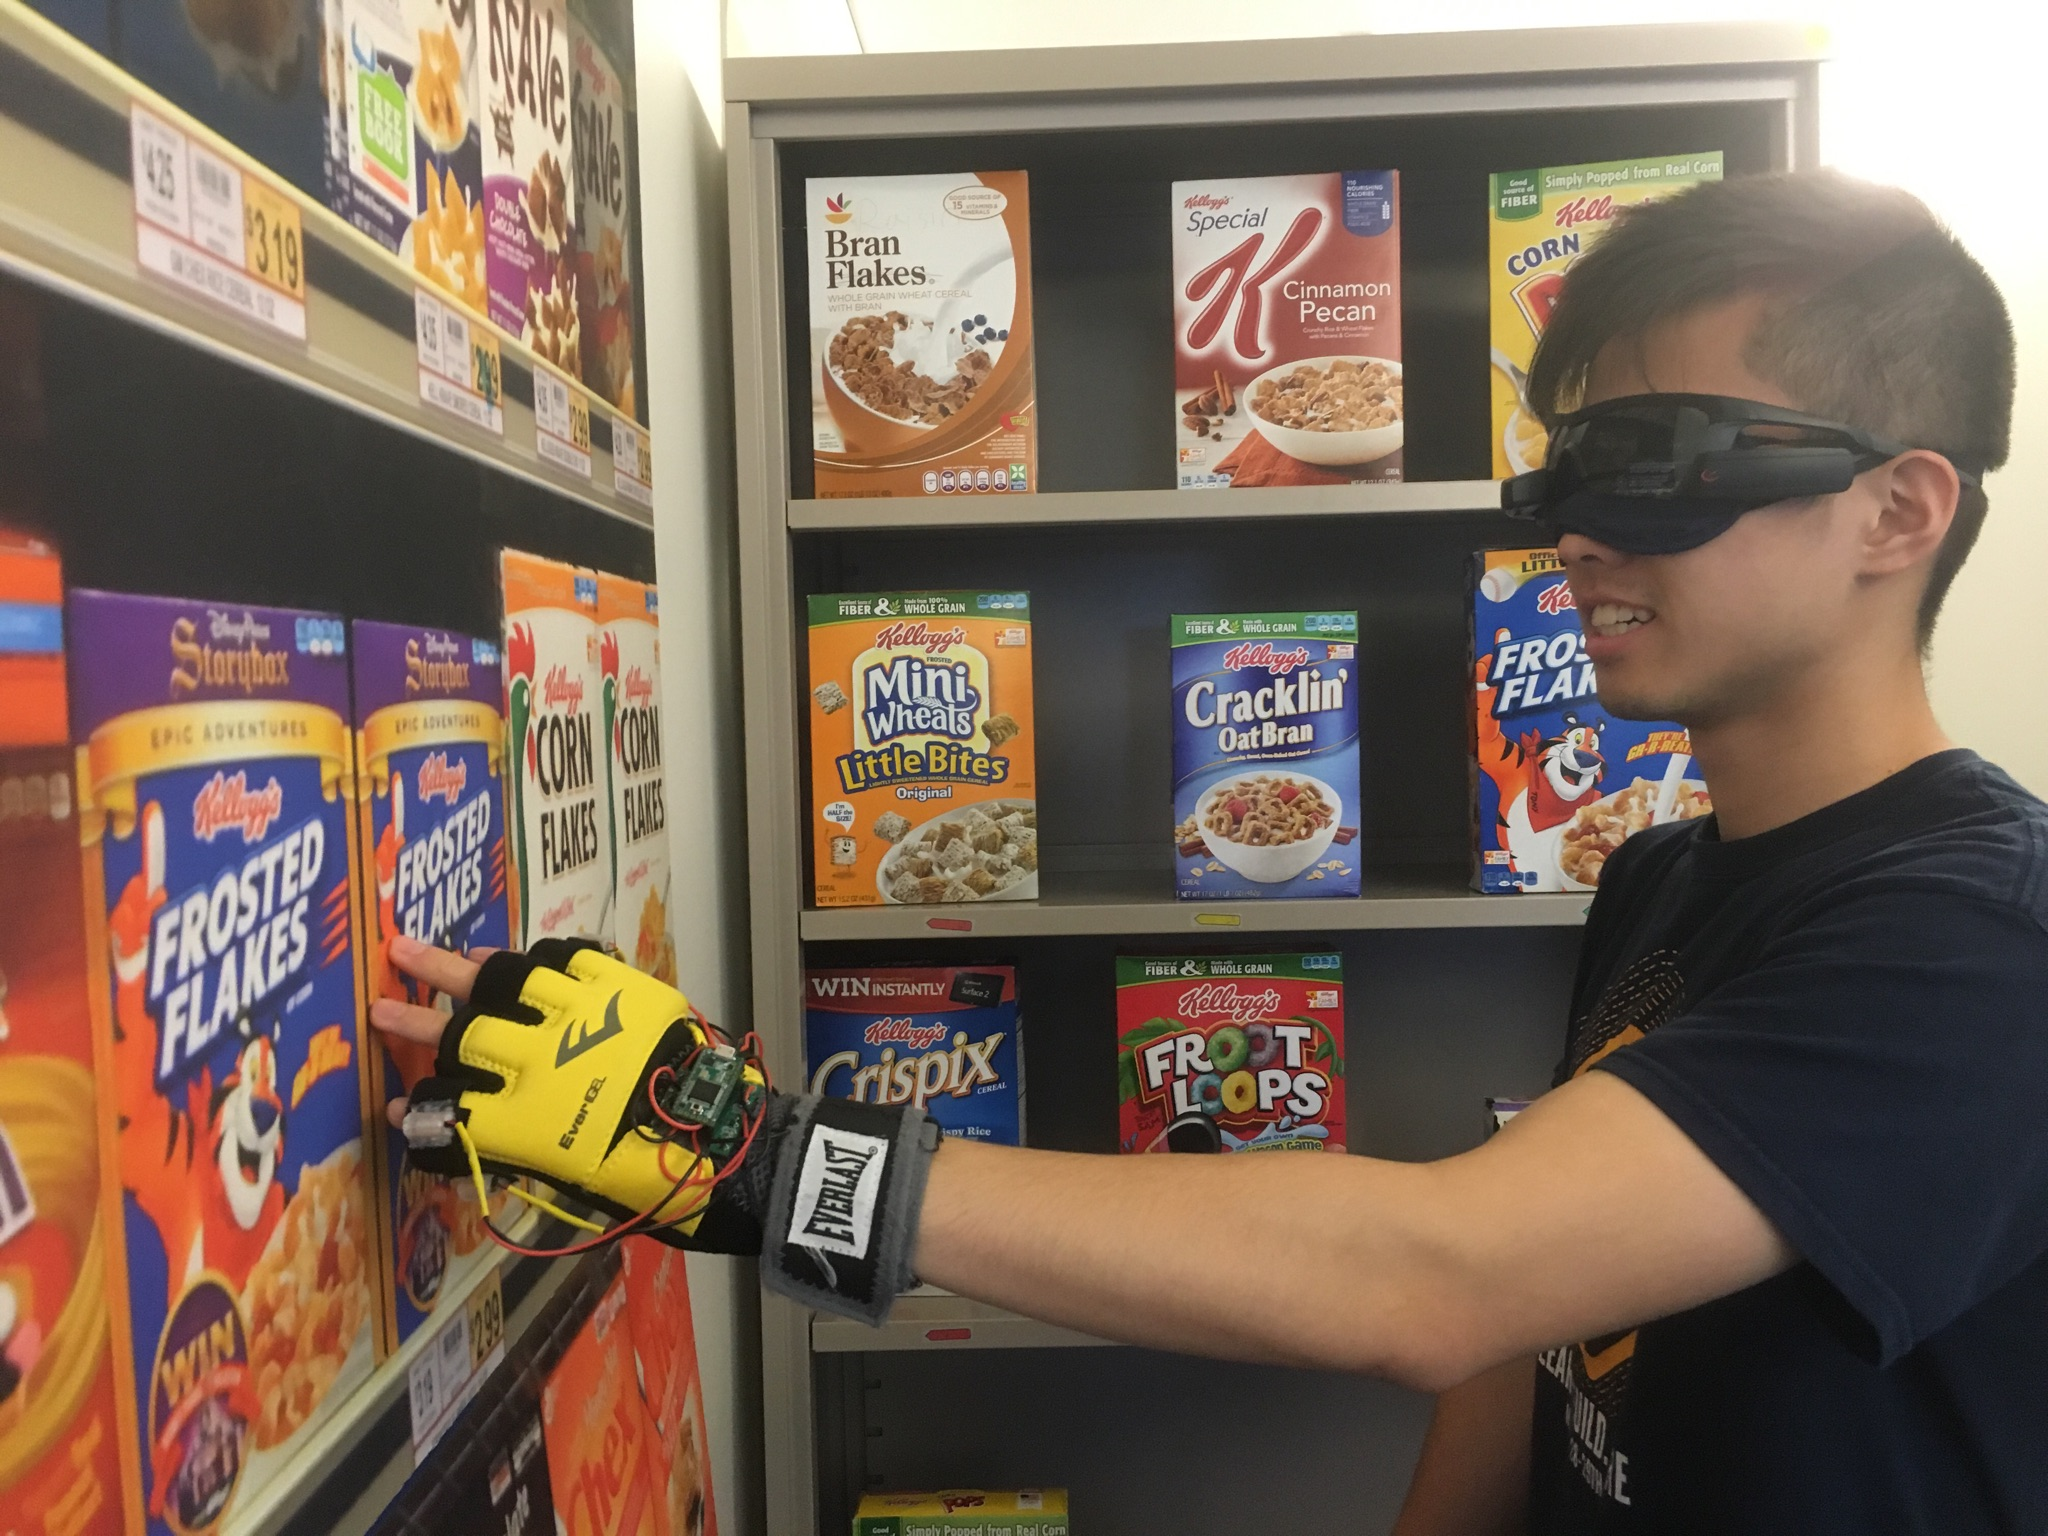
\includegraphics[width=0.9\linewidth,trim={0 0 0 0},clip]{chris_system.jpg}
\caption{ A person using an assistive system using multiple modes of feedback.}
\label{fig:whole_system_chris}
\end{figure}

\subsection{Using the System}
While certain aspects of the system differ across the particular tasks it supports, 
the modes and mechanisms employed during grocery shopping provide good coverage of typical operations, and we describe them in detail below.
In our system, the auditory feedback combined with the haptic feedback from the glove provide the needed assistance to the shopper. 
 
\subsection{Challenges}
Creating a truly assistive system with a variety of interfaces presents a series 
of challenges, not all of which are initially obvious. These challenges include guiding the person
through the store which includes localization, obstacle and person avoidance and grocery shopping. 
Other challenges are user centric. These include adapting the frequency of guidance commands to the speed at which the person is moving, 
reconciling different camera views to provide correct guidance, and having enough computational power to keep the system real-time. 
These challenges can be resolved via various methods. To solve the problem of guiding the person through the store, the smart cart could be equipped with various sensors. 
This could include cameras that not only have RGB information, but even depth and possibly thermal sensors. 
Also the use of localization technologies such as indoor GPS, and bluetooth beacons around the store have the ability to track the user and 
provide the needed level of localization to the system.

Another challenge that arose came from having two camera views that are not always in alignment with one another. An example of when this occurs is 
while shopping when the user goes to grab a product, (s)he might look away while still reaching in towards the intended product. 
This poses a challenge to a system giving guidance based on the view from those cameras. One possible solution to this issue would be the addition of sensors 
to the glasses and the glove. The addition of an IMU and Magnometer to both of the edge compute solutions give the ability to correctly provide guidance in these cases. 
An example how this would work is if the headset camera view indicates the person needed to move right, 
but the glove camera was pointing straight. The system would be able tell the user to turn just their head to align the two views.
The biggest challenge that exists in a guidance system is being able to keep up with the real-time demands of the user. With an assistive system, 
solving this is crucial. In order to do this effectively, the system as a whole must leverage every available compute power 
including that available at both the edge devices, the local infrastructure and a powerful cloud compute platform. 

As stated earlier, for our cloud compute device we use a high-performance server that is enabled with both FPGAs and GPUs. 
By leveraging custom architectures and exploiting parallel algorithms we are able to process 1080p video frames at around 50fps. 
While this may seem like it meets the real-time constraint it does not. Since a server needs to be able handle multiple connections at once, 
just the accelerated back-end would handle 50 streams at 1fps. To make up this gap in performance, 
tricks need to be played at the local and edge compute devices to force this difference to be imperceivable. 
Some of the compute that can be done at the front-end mainly involves the filtering of data. For instance, a local infrastructure would be able to run the 
images being streamed back to the server through one of our hardware accelerated saliency algorithms. Additionally the edge device 
could use its sensors to only send a frame when the user has moved enough that the scene needs to be recomputed fully. 
Once the desired products are found, the local infrastructure or edge device would be able to run a computationally less intense tracking 
algorithm to be able to continue to guide the user toward the product between communications with the cloud back-end.

In the next section we discuss a few algorithms deployed in our recognition system that use techniques to augment machine learning. 



\section{Beyond Deep Learning: Pragmatic Optimizations for Constrained Resources and Limited Time}
\label{sec:vision}
%Deep Learning

%CNNs
Convolutional Neural Networks (CNNs) have become extremely popular and being used to solve a variety of image recognition problems. 
More recent and advanced CNN architectures have become deeper and more complex haing 10 to 20 
layers of Rectified Linear Units, hundreds of millions of weights, and billions of connections between units.
The reader is pointed to ~\cite{Bengio2009} for insights on deep architectures in general and ~\cite{DNNNature2015} for CNN-based learning and their recent advances.

While CNNs are an important thrust of research, they tend to be computationally expensive and deploying them on mobile platforms results in huge memory overheads. 
Another important insight recently unearthed by ~\cite{facenet}, is that the accuracies of CNNs can saturate after a few million images of training data.
Also the overall efficacy of the image recognition pipeline is contingent upon having a good region proposal scheme that feeds regions of interest (RoIs) into the CNN. 
A variety of strategies can be used to augment the capabilities of neural networks and we discuss a few below.

\subsection{Visual Attention}
Humans process only certain streams of visual information depending upon the task at hand. 
From a systems perspective, visual attention can be used as an efficient mechanism to prioritize visual processing.  
Pixel-level saliency models such as Attention by Information Maximiztion (AIM)~\cite{Bruceb} can be used in 
automatic household pantry organization and maintenance, particularly 
as part of visual assist systems for the visually impaired. Computationally, AIM determines visual salience based on the amount of information present in 
local regions of the image within the context of its surrounding region. 
Suppose a product (say cookies) is wrongly placed in a shelf that stores products of another type (say shampoo), the segment of the shelf image containing cookies is 
``less likely'' (higher self-information) to appear in the scene which mostly has image patches of shampoo, 
and therefore it is easily distinguishable or is considered ``salient''. This is shown in Figure~\ref{tab:saliencya}.
Once a salient region is detected, a second stage of object classification can be deployed to identify the wrongly placed object.  

%Saliency App 1
\begin{figure}[!htb]
\centering
\begin{tabular}{@{}l@{} @{}l@{}}
\vspace{-5pt}
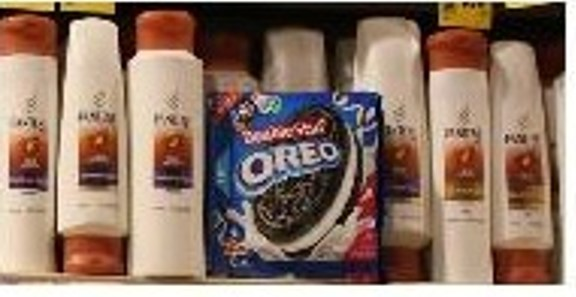
\includegraphics[width=0.5\linewidth,trim={0 0 0 0},clip]{mp1a.jpg} & 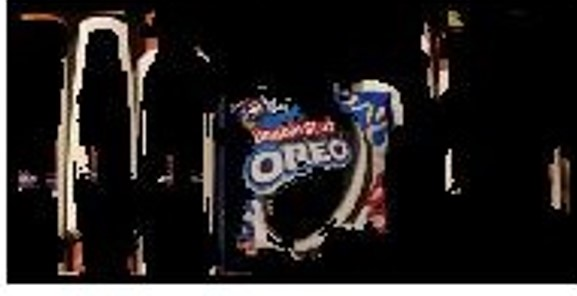
\includegraphics[width=0.5\linewidth,trim={0 0 0 0},clip]{mp1b.jpg}\\[\abovecaptionskip]
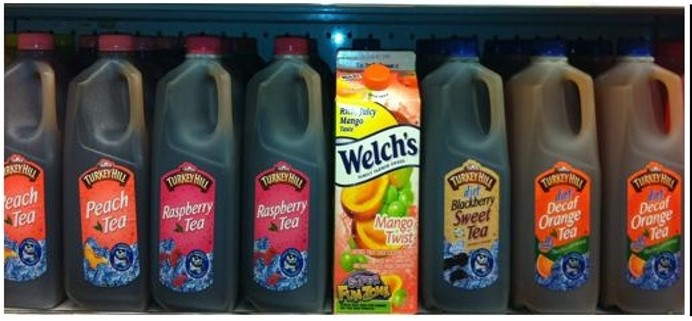
\includegraphics[width=0.5\linewidth,trim={0 0 0 0},clip]{mp2a.jpg} & 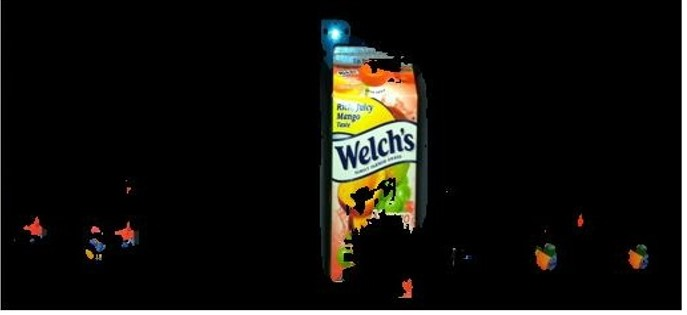
\includegraphics[width=0.5\linewidth,trim={0 0 0 0},clip]{mp2b.jpg}\\[\abovecaptionskip]
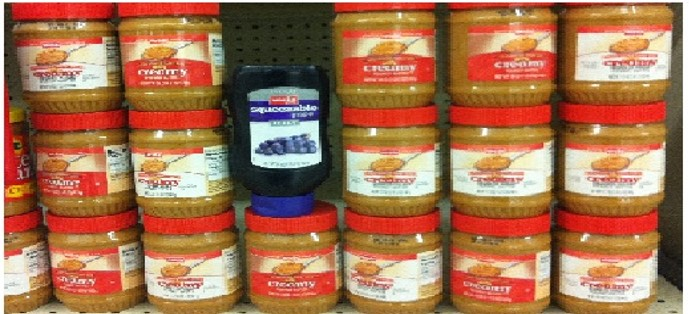
\includegraphics[width=0.5\linewidth,trim={0 0 0 0},clip]{mp3a.jpg} & 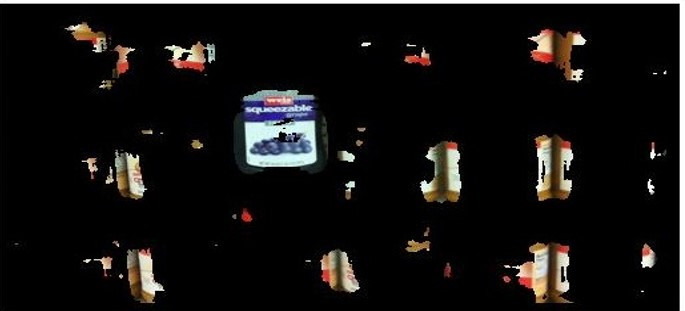
\includegraphics[width=0.5\linewidth,trim={0 0 0 0},clip]{mp3b.jpg}\\[\abovecaptionskip]
\small(a) Original image & \small (b) Thresholded saliency map\\
\end{tabular}
\caption{Saliency used for missplaced item detection.}
\label{tab:saliencya}
\end{figure}

\subsection{Redundancy}
A lot of visual scenes exhibit redundancy in some form or the other. 
For example, in a grocery aisle there are a lot of similar looking products like cereal boxes, detergent bottles, etc. Rather than processing each of these items 
as independent entities, we can localize similar RoIs, run our classification engine on only one of them and then assign the corresponding label to all of the similar 
RoIs. Figure~\ref{tab:saliencyb} illustrates this flow where AIM is used to generate initial seed RoIs that are then coupled with SURF keypoint matching 
to generate a list of RoIs that are similar in structure. 

%Saliency App 2
\begin{figure*}[!htb]
\centering
\begin{tabular}{@{}c@{} @{}c@{} @{}c@{}}
\vspace{-5pt}
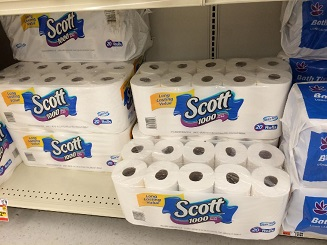
\includegraphics[width=0.32\linewidth,trim={0 0 0 0},clip]{scott_img.jpg} & 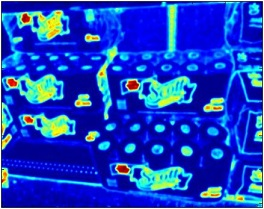
\includegraphics[width=0.31\linewidth,trim={0 0 0 0},clip]{scott_sali.jpg} & 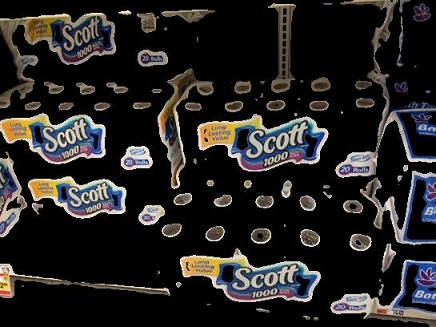
\includegraphics[width=0.32\linewidth,trim={0 0 0 0},clip]{scott_roi.jpg}\\[\abovecaptionskip]
\small(a) Original image & \small (b) Saliency Map & \small (c) Thresholded Map \\
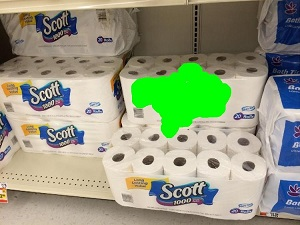
\includegraphics[width=0.32\linewidth,trim={0 0 0 0},clip]{scott_best_roi.jpg} & 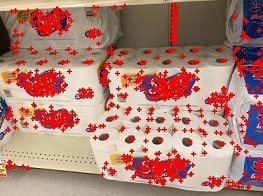
\includegraphics[width=0.32\linewidth,trim={0 0 0 0},clip]{scott_surf2.jpg} & 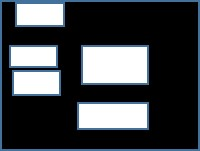
\includegraphics[width=0.32\linewidth,trim={0 0 0 0},clip]{scott_mask.jpg}\\[\abovecaptionskip]
\small(a) Best RoI & \small (b) SURF keypoints & \small (c) Regions of Interest \\
\end{tabular}
\caption{Saliency and SURF used to identify similar items.}
\label{tab:saliencyb}
\end{figure*}

\subsection{Context}
% Hierarchy of Parts
While deep learning models use learnt features to recognize objects in a scene, another contrasting approach is to use graphical models that build hierarchical 
representations of objects~\cite{hop}. Compositional rules can be used to build context cues to recognize objects never seen before. For example, an object having 
four wheels can be classified as a vehicle even if it is a new model of a car. 
% Spatial Context
While CNNs have been widely used for image category recognition, when it comes to recognizing objects in video streams, spatial context can play a huge role in 
reducing the workload on these computationally intensive classifiers. As shown in Figure~\ref{fig:viconet}, visual scenes can be represented as a knowledge graph.   
For example, in ~\cite{estimedia2015}, the authors proposed a Bayesian network called Visual Co-occurrence Network (ViCoNet) to not 
only improve the performance of their system, but also increase the recognition rates.

\begin{figure}[!htb]
\centering
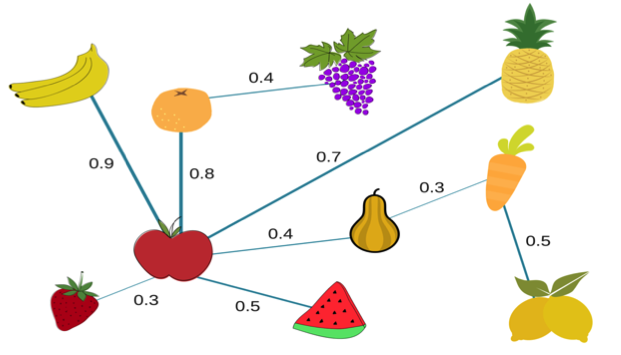
\includegraphics[width=0.9\linewidth]{viconetexample.png}
\caption{Spatial relations exist between frequently co-occurring objects. These relationships can then be used as context cues to guide the classifiers.}
\label{fig:viconet}
\end{figure} 

\subsection{Multimodal Fusion}
Humans use multisensory information from different sensory systems and combine it to influence 
perception, decisions, and overt behavior~\cite{stein2009neural}. Wearables can be used in a similar fashion to help users in different tasks. 
A rich topic of exploration is figuring out a way to fuse multi-sensor information, especially data from vision that is fundamentally two-dimensional with a temporal 
unidimensional stream of data from other sensors to make predictions of the current state of the user. Multi-sensor information coming in from different devices can be 
streamed to distributed networks that can then make real-time updates. In Figure~\ref{tab:sensor}, we illustrate data recorded from a wearable device while two users
walk in three different directions. These sensors are sensitive enough to be used as localization cues. 

%MultiModal Analysis
\begin{figure}[!htb]
\centering
\begin{tabular}{@{}c@{} @{}c@{}}
\vspace{-5pt}
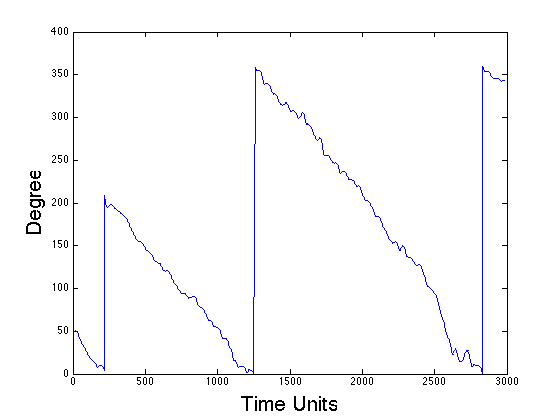
\includegraphics[width=0.5\linewidth,trim={0 0 0 0},clip]{walk_left_p1.png} & 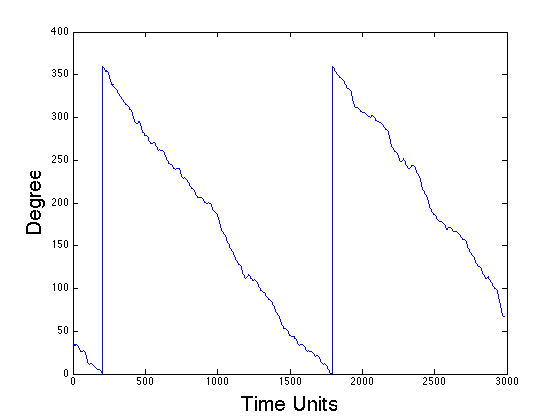
\includegraphics[width=0.5\linewidth,trim={0 0 0 0},clip]{walk_left_p2.png}\\[\abovecaptionskip]
\small(a) Person 1 - Left & \small (b) Person 2 - Left\\
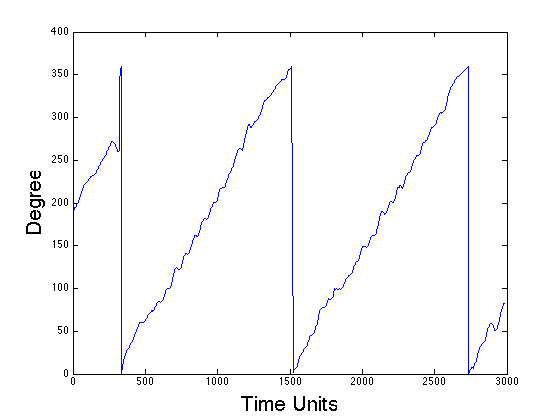
\includegraphics[width=0.5\linewidth,trim={0 0 0 0},clip]{walk_right_p1.png} & 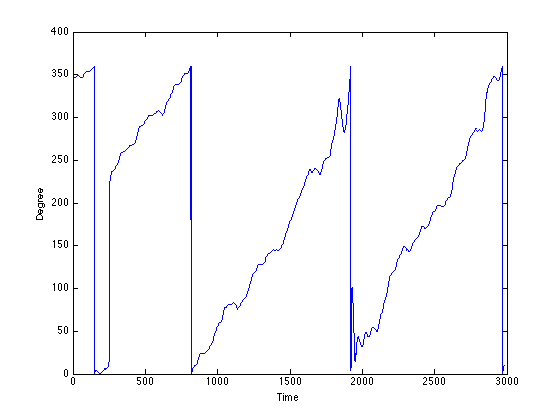
\includegraphics[width=0.5\linewidth,trim={0 0 0 0},clip]{walk_right_p2.png}\\[\abovecaptionskip]
\small(a) Person 1 - Right & \small (b) Person 2 - Right\\
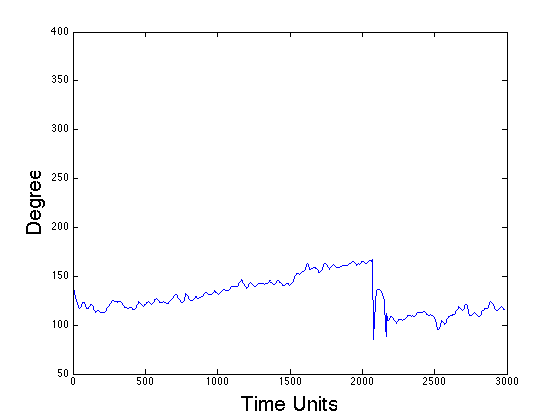
\includegraphics[width=0.5\linewidth,trim={0 0 0 0},clip]{walk_straight_p1.png} & 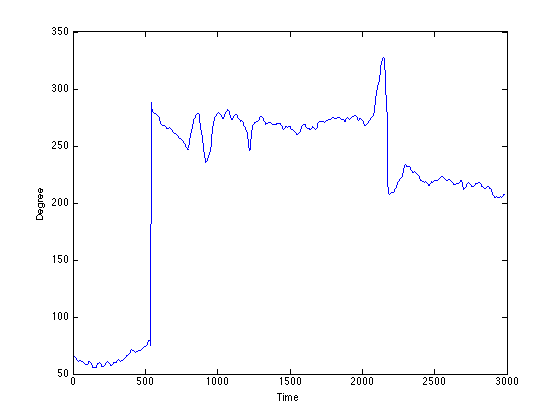
\includegraphics[width=0.5\linewidth,trim={0 0 0 0},clip]{walk_straight_p2.png}\\[\abovecaptionskip]
\small(a) Person 1 - Straight & \small (b) Person 2 - Straight\\
\end{tabular}
\caption{Other sensor information used for localization.}
\label{tab:sensor}
\end{figure}


\section{Hardware Support}
\label{sec:hardware}
\subsection{Custom Chips}

%Coupling structural with learnt features
\begin{figure*}[!htb]
\centering
\begin{tabular}{@{}c@{} @{}c@{} @{}c@{} @{}c@{}}
\vspace{-5pt}

\includegraphics[width=0.25\linewidth,trim={0 0 0 0},clip]{MissingFigure.pdf} & 
\includegraphics[width=0.25\linewidth,trim={0 0 0 0},clip]{MissingFigure.pdf} & 
\includegraphics[width=0.25\linewidth,trim={0 0 0 0},clip]{MissingFigure.pdf} & 
\includegraphics[width=0.25\linewidth,trim={0 0 0 0},clip]{MissingFigure.pdf}\\[\abovecaptionskip]
\small(a) Original image & \small (b) HOG output & \small (c) Reduced threshold HOG output & \small (d) HOG-CNN output \\
\end{tabular}
\caption{Coupling structured features with learnt features}
\label{tab:tn}
\end{figure*}

\subsection{Brain-like Architectures}
As machine learning workloads become more and more involved, modern architectures beyond von-Neumann are being explored.
IBM's TrueNorth chip consists of 4096 neurosynaptic cores arranged in a 2-D
array occupying 4.3 ${cm^2}$ of area in a 28 nm lowpower CMOS process. This brain-like chip consumes merely 65 mW of 
power while running a typical computer vision application~\cite{truenorth}. Having accelerated some of the key computer vision models using custom fabrics 
like FPGAs and GPUs, we are now looking to map them onto TrueNorth. Figure~\ref{tab:tn} shows the output of the HOG-based person detection when modeled for TrueNorth. 

%TN
\begin{figure*}[!htb]
\centering
%\def\arraystretch{1.5} %
\begin{tabular}{@{}c@{} @{\hspace{2em}}c@{} @{\hspace{2em}}c@{}}
\vspace{-5pt}
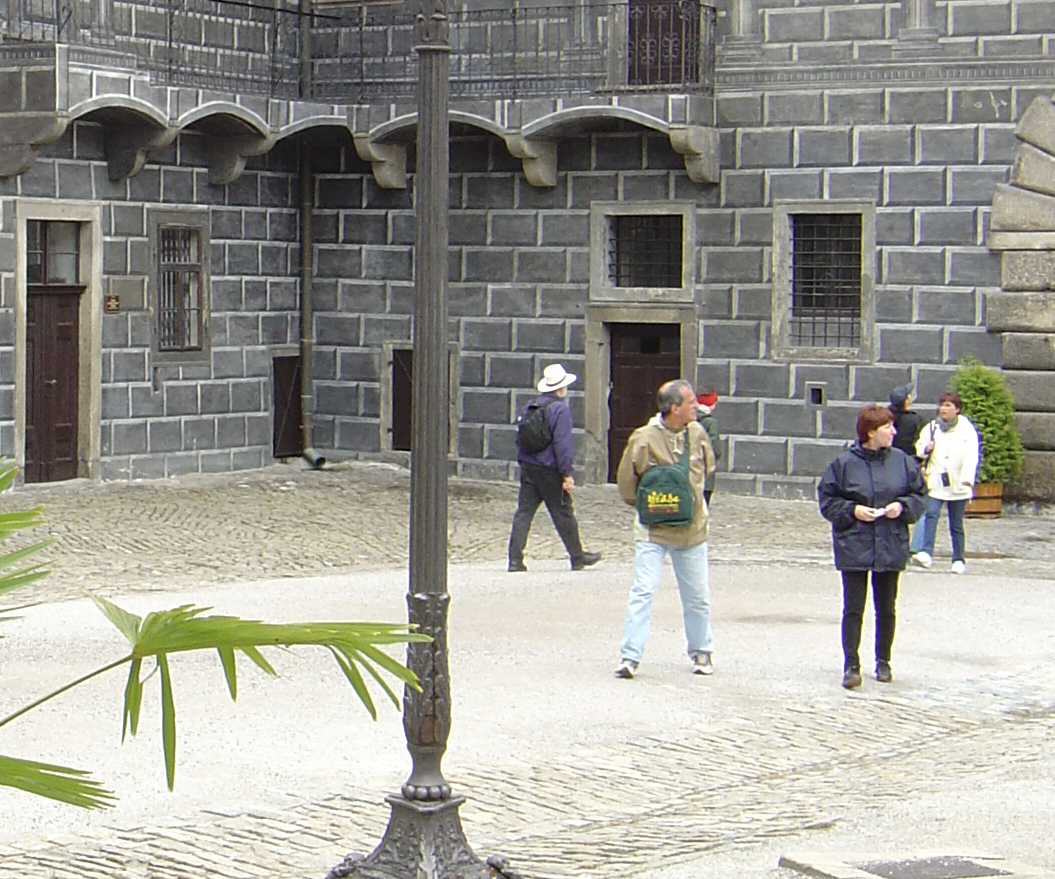
\includegraphics[width=0.29\linewidth,trim={0 0 0 0},clip]{tn_input_46.png} & 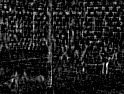
\includegraphics[width=0.32\linewidth,trim={0 0 0 0},clip]{tn_dotp_46.jpg} & 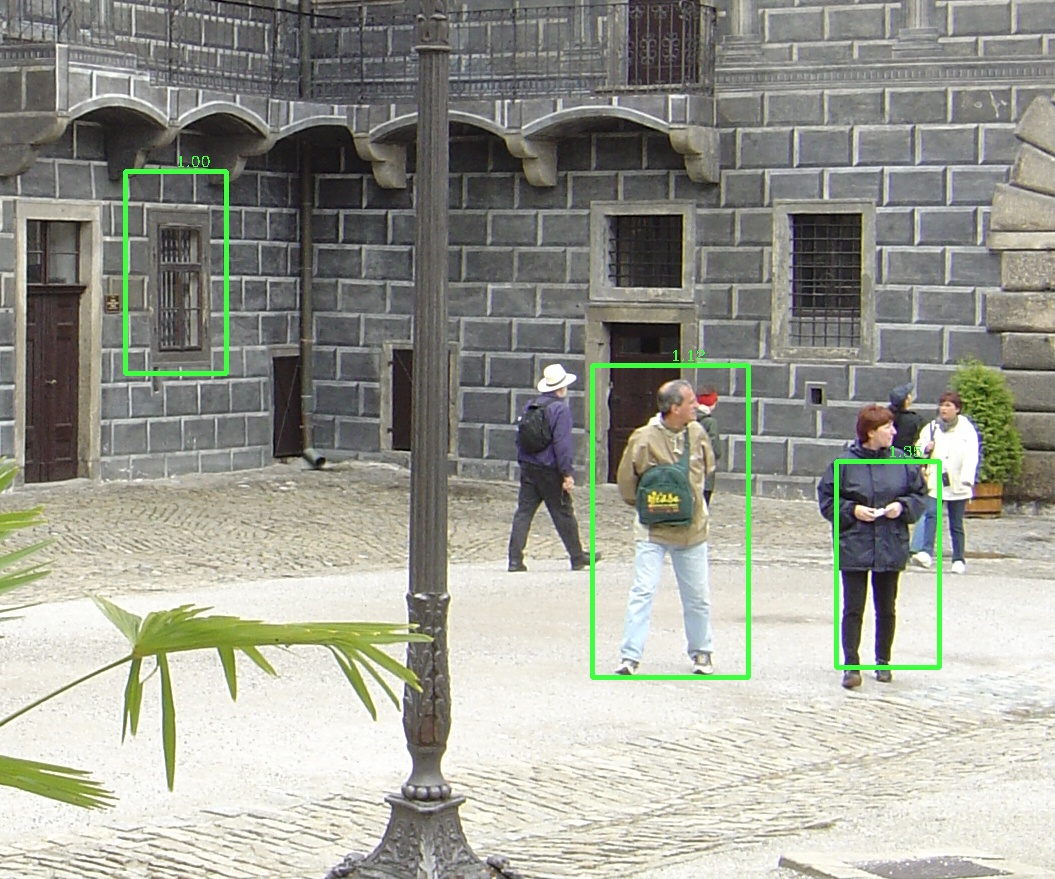
\includegraphics[width=0.29\linewidth,trim={0 0 0 0},clip]{tn_detection_46.jpg}\\[\abovecaptionskip]
\small(a) Original image & \small (b) Dot Product & \small (c) Detections \\
\end{tabular}
\caption{Mapping HOG to True North}
\label{tab:tn}
\end{figure*}

\subsection{Emerging Devices}



\section{Conclusion}
\label{sec:conclusion}
This work highlighted the efficacy of personal visual assist systems in our day to day activities. 
More specifically, the design and integration of a multi-task grocery assist system for the visually impaired was 
discussed. We also introduced the latest architectures and emerging devices that are being explored to further improve the capabilities of such systems. 
%As technological advances spur growth, more and more consumer products will become available. 




%\hfill mds
 
%\hfill September 17, 2014

%\subsection{Subsection Heading Here}
%Subsection text here.

% needed in second column of first page if using \IEEEpubid
%\IEEEpubidadjcol

%\subsubsection{Subsubsection Heading Here}
%Subsubsection text here.


% An example of a floating figure using the graphicx package.
% Note that \label must occur AFTER (or within) \caption.
% For figures, \caption should occur after the \includegraphics.
% Note that IEEEtran v1.7 and later has special internal code that
% is designed to preserve the operation of \label within \caption
% even when the captionsoff option is in effect. However, because
% of issues like this, it may be the safest practice to put all your
% \label just after \caption rather than within \caption{}.
%
% Reminder: the "draftcls" or "draftclsnofoot", not "draft", class
% option should be used if it is desired that the figures are to be
% displayed while in draft mode.
%
%\begin{figure}[!t]
%\centering
%\includegraphics[width=2.5in]{myfigure}
% where an .eps filename suffix will be assumed under latex, 
% and a .pdf suffix will be assumed for pdflatex; or what has been declared
% via \DeclareGraphicsExtensions.
%\caption{Simulation results for the network.}
%\label{fig_sim}
%\end{figure}

% Note that IEEE typically puts floats only at the top, even when this
% results in a large percentage of a column being occupied by floats.


% An example of a double column floating figure using two subfigures.
% (The subfig.sty package must be loaded for this to work.)
% The subfigure \label commands are set within each subfloat command,
% and the \label for the overall figure must come after \caption.
% \hfil is used as a separator to get equal spacing.
% Watch out that the combined width of all the subfigures on a 
% line do not exceed the text width or a line break will occur.
%
%\begin{figure*}[!t]
%\centering
%\subfloat[Case I]{\includegraphics[width=2.5in]{box}%
%\label{fig_first_case}}
%\hfil
%\subfloat[Case II]{\includegraphics[width=2.5in]{box}%
%\label{fig_second_case}}
%\caption{Simulation results for the network.}
%\label{fig_sim}
%\end{figure*}
%
% Note that often IEEE papers with subfigures do not employ subfigure
% captions (using the optional argument to \subfloat[]), but instead will
% reference/describe all of them (a), (b), etc., within the main caption.
% Be aware that for subfig.sty to generate the (a), (b), etc., subfigure
% labels, the optional argument to \subfloat must be present. If a
% subcaption is not desired, just leave its contents blank,
% e.g., \subfloat[].


% An example of a floating table. Note that, for IEEE style tables, the
% \caption command should come BEFORE the table and, given that table
% captions serve much like titles, are usually capitalized except for words
% such as a, an, and, as, at, but, by, for, in, nor, of, on, or, the, to
% and up, which are usually not capitalized unless they are the first or
% last word of the caption. Table text will default to \footnotesize as
% IEEE normally uses this smaller font for tables.
% The \label must come after \caption as always.
%
%\begin{table}[!t]
%% increase table row spacing, adjust to taste
%\renewcommand{\arraystretch}{1.3}
% if using array.sty, it might be a good idea to tweak the value of
% \extrarowheight as needed to properly center the text within the cells
%\caption{An Example of a Table}
%\label{table_example}
%\centering
%% Some packages, such as MDW tools, offer better commands for making tables
%% than the plain LaTeX2e tabular which is used here.
%\begin{tabular}{|c||c|}
%\hline
%One & Two\\
%\hline
%Three & Four\\
%\hline
%\end{tabular}
%\end{table}


% Note that the IEEE does not put floats in the very first column
% - or typically anywhere on the first page for that matter. Also,
% in-text middle ("here") positioning is typically not used, but it
% is allowed and encouraged for Computer Society conferences (but
% not Computer Society journals). Most IEEE journals/conferences use
% top floats exclusively. 
% Note that, LaTeX2e, unlike IEEE journals/conferences, places
% footnotes above bottom floats. This can be corrected via the
% \fnbelowfloat command of the stfloats package.


% if have a single appendix:
%\appendix[Proof of the Zonklar Equations]
% or
%\appendix  % for no appendix heading
% do not use \section anymore after \appendix, only \section*
% is possibly needed

% use appendices with more than one appendix
% then use \section to start each appendix
% you must declare a \section before using any
% \subsection or using \label (\appendices by itself
% starts a section numbered zero.)
%


%\appendices
%\section{Proof of the First Zonklar Equation}
%Appendix one text goes here.

% you can choose not to have a title for an appendix
% if you want by leaving the argument blank
\section{}
%Appendix two text goes here.


% use section* for acknowledgment
\section*{Acknowledgment}
This work was supported in part by NSF Expeditions in Computing
Program: Visual Cortex on Silicon CCF 1317560. We acknowledge all
collaborators and participants of the Center whose work has influenced
this article.

% Can use something like this to put references on a page
% by themselves when using endfloat and the captionsoff option.
\ifCLASSOPTIONcaptionsoff
  \newpage
\fi



% trigger a \newpage just before the given reference
% number - used to balance the columns on the last page
% adjust value as needed - may need to be readjusted if
% the document is modified later
%\IEEEtriggeratref{8}
% The "triggered" command can be changed if desired:
%\IEEEtriggercmd{\enlargethispage{-5in}}

% references section

% can use a bibliography generated by BibTeX as a .bbl file
% BibTeX documentation can be easily obtained at:
% http://www.ctan.org/tex-archive/biblio/bibtex/contrib/doc/
% The IEEEtran BibTeX style support page is at:
% http://www.michaelshell.org/tex/ieeetran/bibtex/
\bibliographystyle{IEEEtran}
% argument is your BibTeX string definitions and bibliography database(s)
\bibliography{IEEEabrv,library}
%
% <OR> manually copy in the resultant .bbl file
% set second argument of \begin to the number of references
% (used to reserve space for the reference number labels box)
%\begin{thebibliography}{1}

%\bibitem{IEEEhowto:kopka}
%H.~Kopka and P.~W. Daly, \emph{A Guide to \LaTeX}, 3rd~ed.\hskip 1em plus
%  0.5em minus 0.4em\relax Harlow, England: Addison-Wesley, 1999.

%\end{thebibliography}

% biography section
% 
% If you have an EPS/PDF photo (graphicx package needed) extra braces are
% needed around the contents of the optional argument to biography to prevent
% the LaTeX parser from getting confused when it sees the complicated
% \includegraphics command within an optional argument. (You could create
% your own custom macro containing the \includegraphics command to make things
% simpler here.)
%\begin{IEEEbiography}[{\includegraphics[width=1in,height=1.25in,clip,keepaspectratio]{mshell}}]{Michael Shell}
% or if you just want to reserve a space for a photo:
\vspace{-11mm}
\begin{IEEEbiographynophoto}{Peter A. Zientara} (paz117@cse.psu.edu)
received the B.S. degree in computer engineering from the York College of Pennsylvania in 2014 and is currently pursuing his Ph.D. in computer science and engineering from the the Pennsylvania State University. His research interests are in smart sensors, hardware acceleration, and embedded vision systems.
\end{IEEEbiographynophoto}
\vspace{-12mm}
\begin{IEEEbiographynophoto}{Siddharth Advani} (ska130@cse.psu.edu)
received the B.S. degree in electronics engineering from the Pune University, India in 2005, the M.S. degree in electrical engineering from the Pennsylvania State University in 2009 and the Ph.D. in computer science and engineering from the Pennsylvania State University in 2016. His research interests 
include embedded vision design for smart mobile applications targetted for domain-specific applications.
\end{IEEEbiographynophoto}
\vspace{-12mm}
\begin{IEEEbiographynophoto}{Nikhil Shukla} (nshukla@nd.edu)
received the B.S. degree in electronics
and telecommunications engineering from the
University of Mumbai, India in 2010. He
is currently working toward the Ph.D. degree in
electrical engineering at the University of Notre Dame. 
\end{IEEEbiographynophoto}
\vspace{-12mm}
\begin{IEEEbiographynophoto}{Ikenna Okafor} (izo5011@cse.psu.edu)
is currently in the Integrated Undergraduate program for computer engineering at the Pennsylvania State University. His research interests 
include hardware acceleration for neuromorphic vision algorithms.
\end{IEEEbiographynophoto}
\vspace{-12mm}
\begin{IEEEbiographynophoto}{Kevin Irick} (kevin.irick@siliconscapes.net)
is the CEO and Founder of SiliconScapes LLC based in State College, Pennsylvania. Kevin founded SiliconScapes with the objective to 
develop high-performance, embedded and cloud-based, video analytics systems for security, surveillance and retail applications. Kevin conferred the 
Doctoral degree in computer science and engineering from the Pennsylvania State University in 2009.
His research activities included application-specific hardware accelerator design methodology, hardware-assisted image processing and recognition, 
and high performance computing on reconfigurable architectures.
\end{IEEEbiographynophoto}
\vspace{-12mm}
\begin{IEEEbiographynophoto}{John (Jack) Sampson} (sampson@cse.psu.edu)
received the B.S. degree in electrical engineering and computer science from the University of California, Berkeley in 2002 
and the Ph.D. in computer engineering from the University of California, San Diego in 2010. 
He is an currently an Assistant Professor with the Department of Computer Science and Engineering at the Pennsylvania State University.
His research interests include energy-efficient computing, architectural adaptations to exploit emerging technologies, and mitigating the 
impact of Dark Silicon.
\end{IEEEbiographynophoto}
\vspace{-12mm}
\begin{IEEEbiographynophoto}{Suman Datta} (Suman.Datta.1@nd.edu)
received the B.S. degree in
electrical engineering from the Indian Institute of
Technology, Kanpur, India, in 1995, and the Ph.D.
degree in electrical and computer engineering from
the University of Cincinnati, Cincinnati, OH, USA,
in 1999. From 1999 to 2007, he was a member
of the Logic Technology Development Group, Intel
Corporation. He is currently a Professor
of Electrical Engineering at the University of Notre Dame and 
his group is exploring new materials and novel device architecture for
CMOS enhancement and replacement for future energy-efficient computing applications.
\end{IEEEbiographynophoto}
% insert where needed to balance the two columns on the last page with
% biographies
%\newpage
\vspace{-12mm}
%\begin{IEEEbiography}[{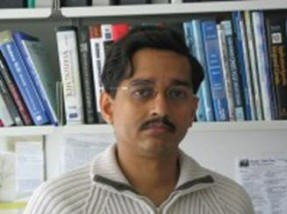
\includegraphics[width=1in,clip,keepaspectratio]{bios/vijay.jpg}}]{Vijaykrishnan Narayanan}
\begin{IEEEbiographynophoto}{Vijaykrishnan Narayanan} (vijay@cse.psu.edu)
received the B.S. degree in computer science and Engineering from the University of Madras, India, in 1993 and the Ph.D. in computer science and engineering 
from the University of South Florida, Tampa, USA, in 1998. He is currently a Professor of Computer Science \& Engineering and Electrical Engineering at the 
Pennsylvania State University. His research interests include power-aware and reliable systems, embedded systems, 
nanoscale devices and interactions with system architectures, reconfigurable systems, computer architectures, network-on-chips, domain-specific computing. 
\end{IEEEbiographynophoto}

% You can push biographies down or up by placing
% a \vfill before or after them. The appropriate
% use of \vfill depends on what kind of text is
% on the last page and whether or not the columns
% are being equalized.

%\vfill

% Can be used to pull up biographies so that the bottom of the last one
% is flush with the other column.
%\enlargethispage{-5in}



% that's all folks
\end{document}


